\documentclass{article}
\usepackage[ipa]{luatexja-preset}
\usepackage{graphicx}
\usepackage{tikz}
\usepackage{bm}
\usetikzlibrary{intersections,calc,arrows.meta,decorations.pathreplacing}
\title{数学図案集}
\author{加藤公一 Kimikazu KATO}

\begin{document}
\maketitle
\section{三角関数}
\begin{figure}\caption{$\sin$と$\cos$の定義(その1)}
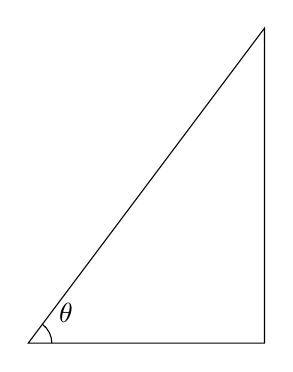
\begin{tikzpicture}
  \draw(0,0)--(3,0)--(3,4)--cycle;
  \draw(0.3,0)arc(0:{atan(4/3)}:0.3)node[midway, above right]{$\theta$};
\end{tikzpicture}
\end{figure}
\begin{figure}\caption{$\sin$と$\cos$の定義(その2)}
\begin{tikzpicture}
  \def\a{55}
  \draw(0,0) circle(2);
  \draw(0,0)-- ++(\a:2)node[right]{$(\cos\theta,\sin\theta)$};
  \draw[->](-3,0)--(3,0)node[right]{$x$};
  \draw[-Stealth](0,-3)--(0,3)node[above]{$y$};
  \draw(0,0)node[below left]{0};
  \draw(0.3,0)arc(0:\a:0.3)node[midway, above right=0mm]{$\theta$};
  \fill(\a:2)circle(2pt);
  \draw(2,0)node[below right]{$1$};
\end{tikzpicture}
\end{figure}
\begin{figure}\caption{正弦定理}
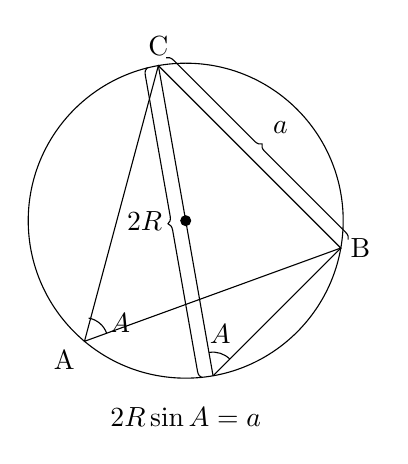
\begin{tikzpicture}
  \draw(0,0) circle(2);
  \draw(-130:2)node[below left]{A}--(-10:2)node[right]{B}
  --(100:2)node[midway, above right=5pt]{$a$}node[above]{C}
  --cycle;
  \draw(100:2)--(-80:2)node[midway, left=5pt]{$2R$};
  \draw(-10:2)--(-80:2);
  \draw[decorate, decoration={brace, raise=4pt}](-80:2)--(100:2);
  \draw[decorate, decoration={brace, raise=4pt}](100:2)--(-10:2);
  \draw($(-80:2)+({0.3*cos(45)},{0.3*sin(45)})$)arc(45:100:0.3)
  node[midway, above]{$A$};
  \draw($(-130:2)+({0.3*cos(20)},{0.3*sin(20)})$)arc(20:80:0.3)
  node[midway, right]{$A$};
  \fill(0,0)circle(2pt);
  \draw(0,-2.5)node{$2R\sin A=a$};
\end{tikzpicture}
\end{figure}
\end{document}
